\documentclass[11pt]{article}
\usepackage[textwidth=18.0cm, textheight=23.0cm, top=2.0cm]{geometry}
\usepackage{pst-all}
\usepackage{amssymb}
\usepackage{tikz}
\usepackage{underscore}\begin{document}
\pagestyle{empty}


ClassName: \underline{\textbf{Class_08.2bp-15}}
\par
BinSize: \underline{\textbf{100 × 100}}
\par
ReduceSize: \underline{\textbf{100 × 100}}
\par
TypeNum: \underline{\textbf{40}}
\par
Num: \underline{\textbf{40}}
\par
OutS: \underline{\textbf{120000}}
\par
InS: \underline{\textbf{94805}}
\par
Rate: \underline{\textbf{0.790}}
\par
UB: \underline{\textbf{12}}
\par
LB0: \underline{\textbf{12}}
\par
LB: \underline{\textbf{12}}
\par
LBWithCut: \underline{\textbf{12}}
\par
NodeCut: \underline{\textbf{0}}
\par
ExtendedNodeCnt: \underline{\textbf{1}}
\par
GenNodeCnt: \underline{\textbf{1}}
\par
PrimalNode: \underline{\textbf{0}}
\par
ColumnCount: \underline{\textbf{12}}
\par
TotalCutCount: \underline{\textbf{0}}
\par
RootCutCount: \underline{\textbf{0}}
\par
LPSolverCnt: \underline{\textbf{1}}
\par
PricingSolverCnt: \underline{\textbf{0}}
\par
BranchAndBoundNum: \underline{\textbf{1}}
\par
isOpt: \underline{\textbf{true}}
\par
TimeOnPrimal: \underline{\textbf{0.000 s}}
\par
TimeOnPricing: \underline{\textbf{0.000 s}}
\par
TimeOnRmp: \underline{\textbf{0.062 s}}
\par
TotalTime: \underline{\textbf{0.125 s}}
\par
\newpage


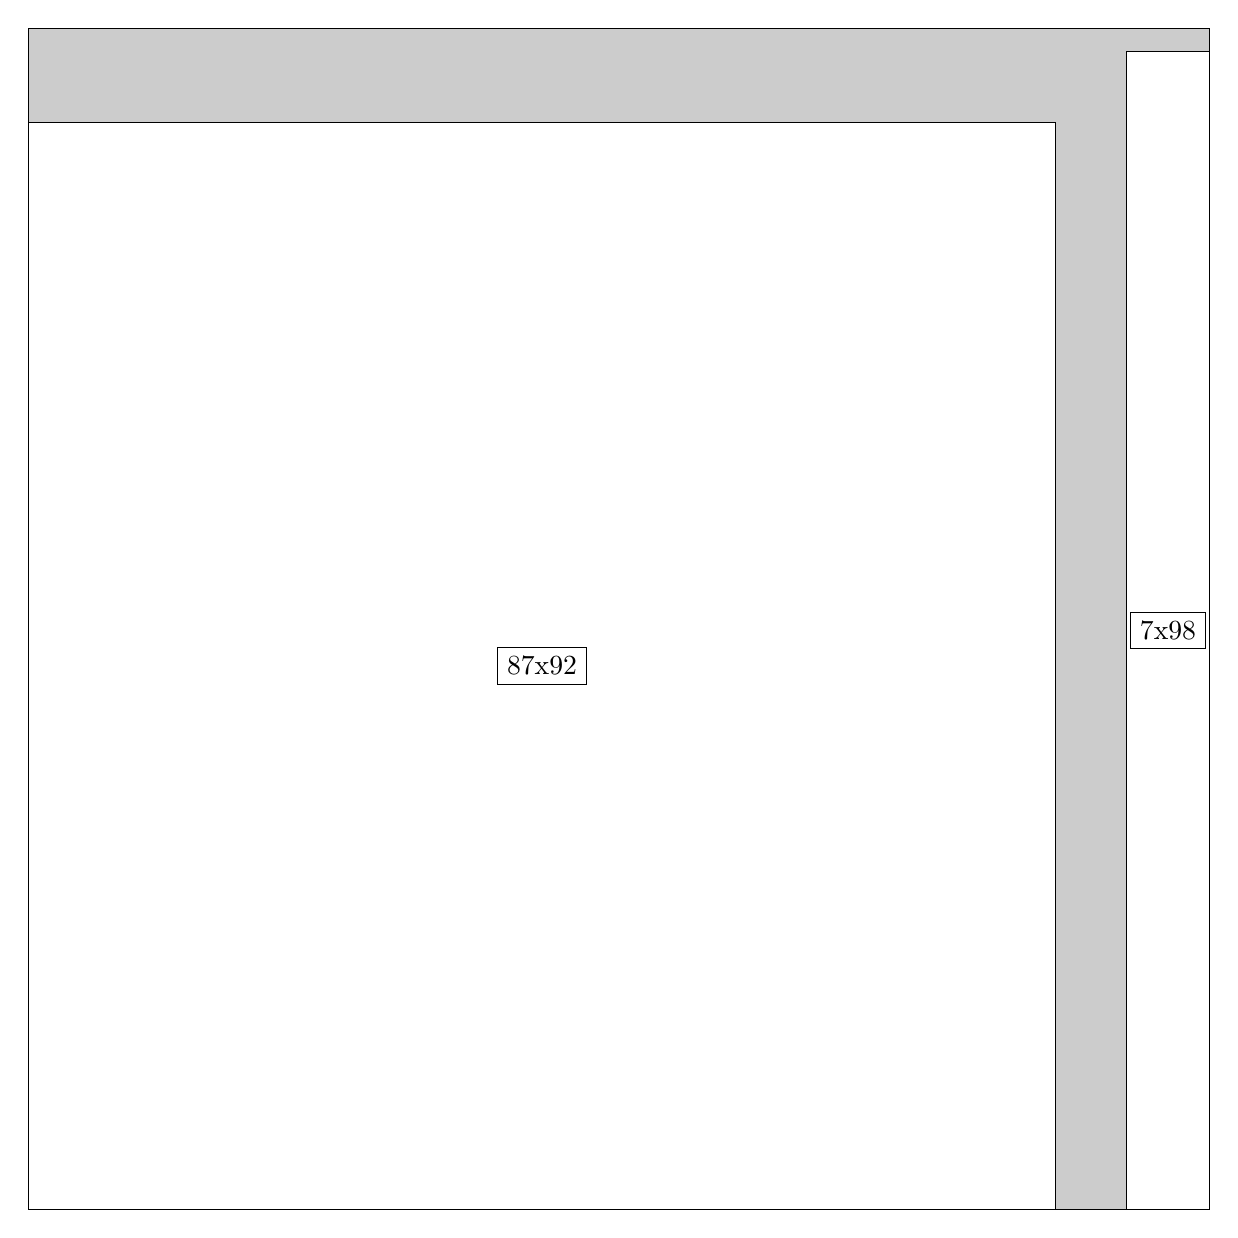
\begin{tikzpicture}[shorten >=1pt,scale=1.0,every node/.style={scale=1.0},->]
\tikzstyle{vertex}=[circle,fill=black!25,minimum size=14pt,inner sep=0pt]
\filldraw[fill=gray!40!white, draw=black] (0,0) rectangle (15.0,15.0);
\foreach \name/\x/\y/\w/\h in {87x92/0.0/0.0/13.049999999999999/13.799999999999999,7x98/13.95/0.0/1.05/14.7}
\filldraw[fill=white!40!white, draw=black] (\x,\y) rectangle node[draw] (\name) {\name} ++(\w,\h);
\end{tikzpicture}


w =87 , h =92 , x =0 , y =0 , v =8004
\par
w =7 , h =98 , x =93 , y =0 , v =686
\par
\newpage


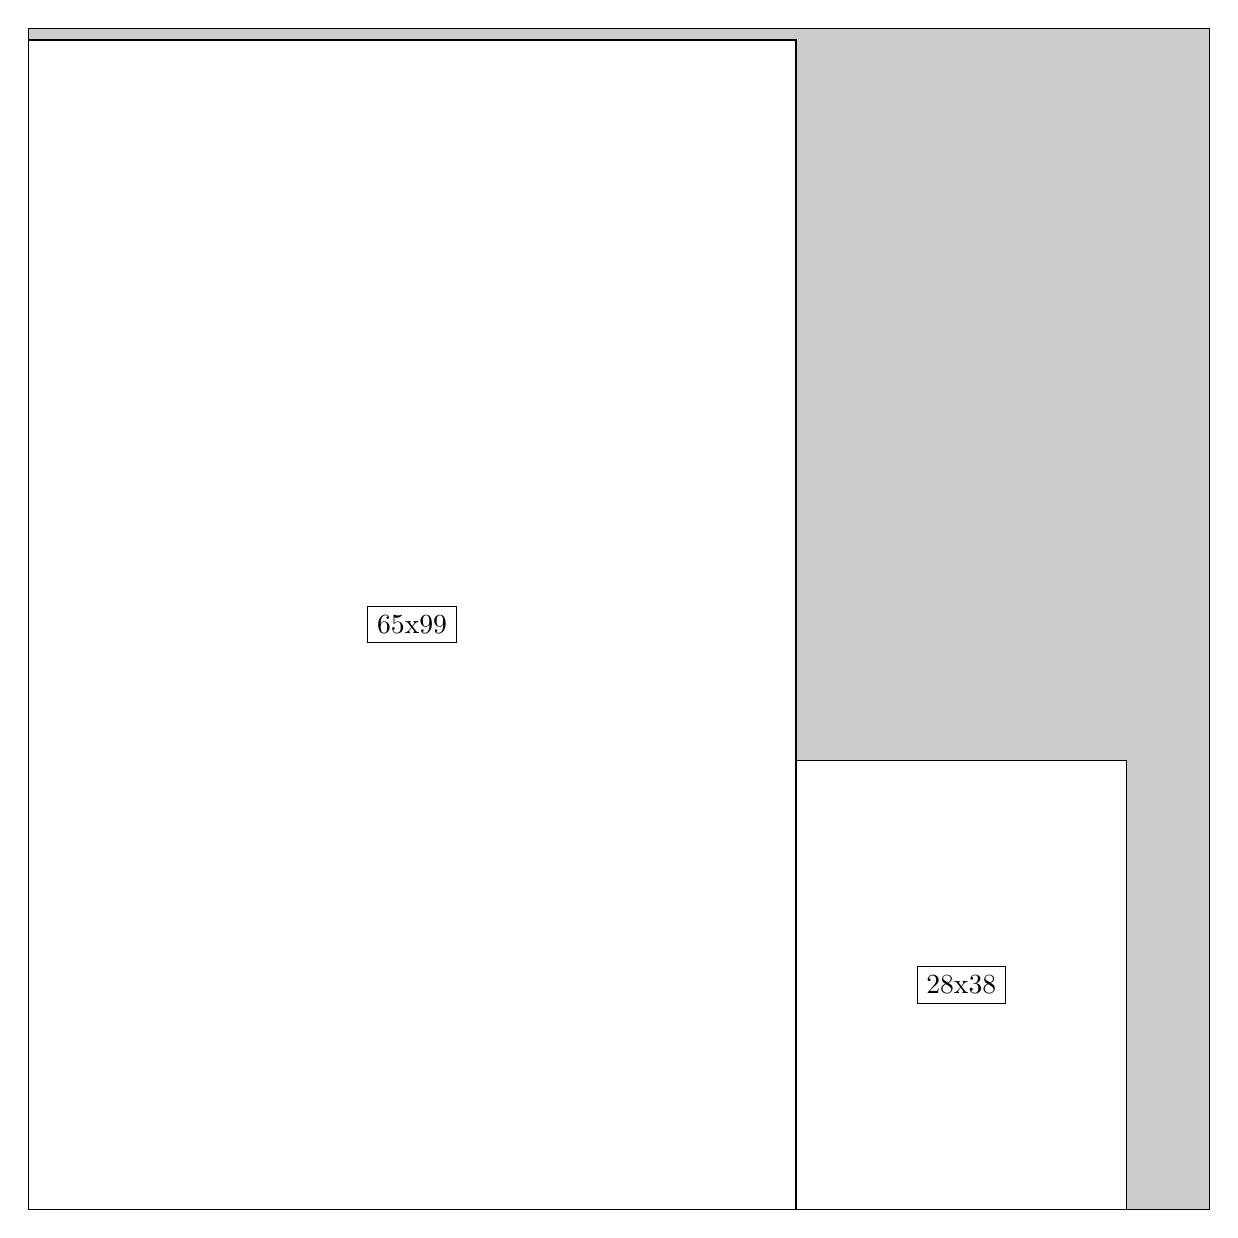
\begin{tikzpicture}[shorten >=1pt,scale=1.0,every node/.style={scale=1.0},->]
\tikzstyle{vertex}=[circle,fill=black!25,minimum size=14pt,inner sep=0pt]
\filldraw[fill=gray!40!white, draw=black] (0,0) rectangle (15.0,15.0);
\foreach \name/\x/\y/\w/\h in {65x99/0.0/0.0/9.75/14.85,28x38/9.75/0.0/4.2/5.7}
\filldraw[fill=white!40!white, draw=black] (\x,\y) rectangle node[draw] (\name) {\name} ++(\w,\h);
\end{tikzpicture}


w =65 , h =99 , x =0 , y =0 , v =6435
\par
w =28 , h =38 , x =65 , y =0 , v =1064
\par
\newpage


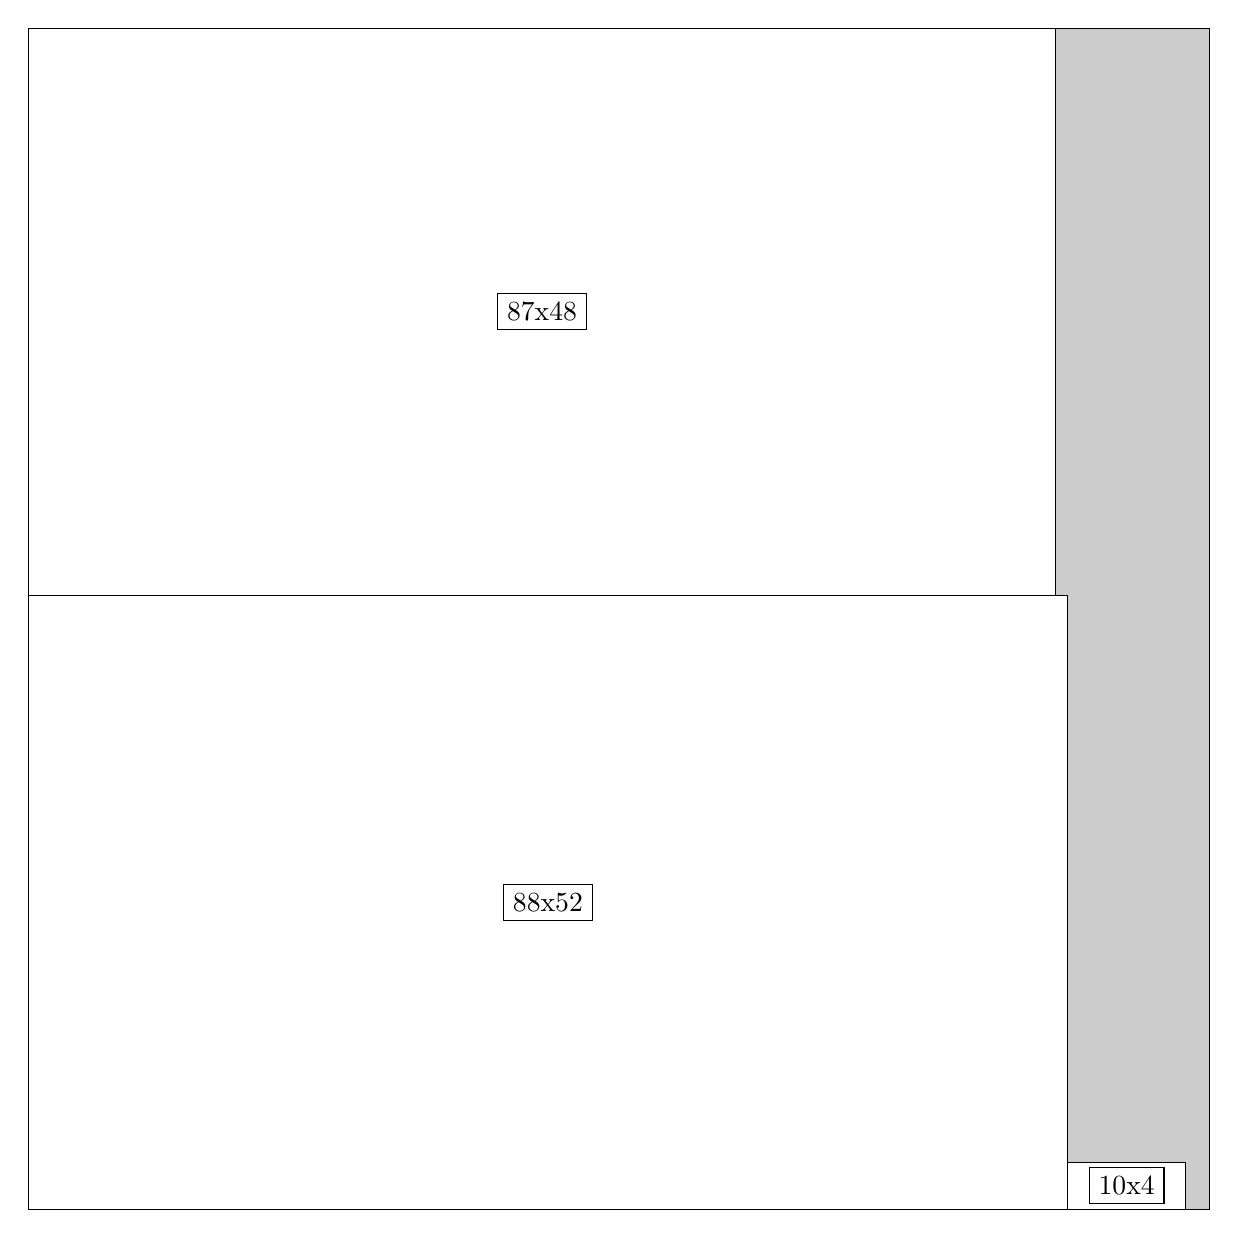
\begin{tikzpicture}[shorten >=1pt,scale=1.0,every node/.style={scale=1.0},->]
\tikzstyle{vertex}=[circle,fill=black!25,minimum size=14pt,inner sep=0pt]
\filldraw[fill=gray!40!white, draw=black] (0,0) rectangle (15.0,15.0);
\foreach \name/\x/\y/\w/\h in {88x52/0.0/0.0/13.2/7.8,87x48/0.0/7.8/13.049999999999999/7.199999999999999,10x4/13.2/0.0/1.5/0.6}
\filldraw[fill=white!40!white, draw=black] (\x,\y) rectangle node[draw] (\name) {\name} ++(\w,\h);
\end{tikzpicture}


w =88 , h =52 , x =0 , y =0 , v =4576
\par
w =87 , h =48 , x =0 , y =52 , v =4176
\par
w =10 , h =4 , x =88 , y =0 , v =40
\par
\newpage


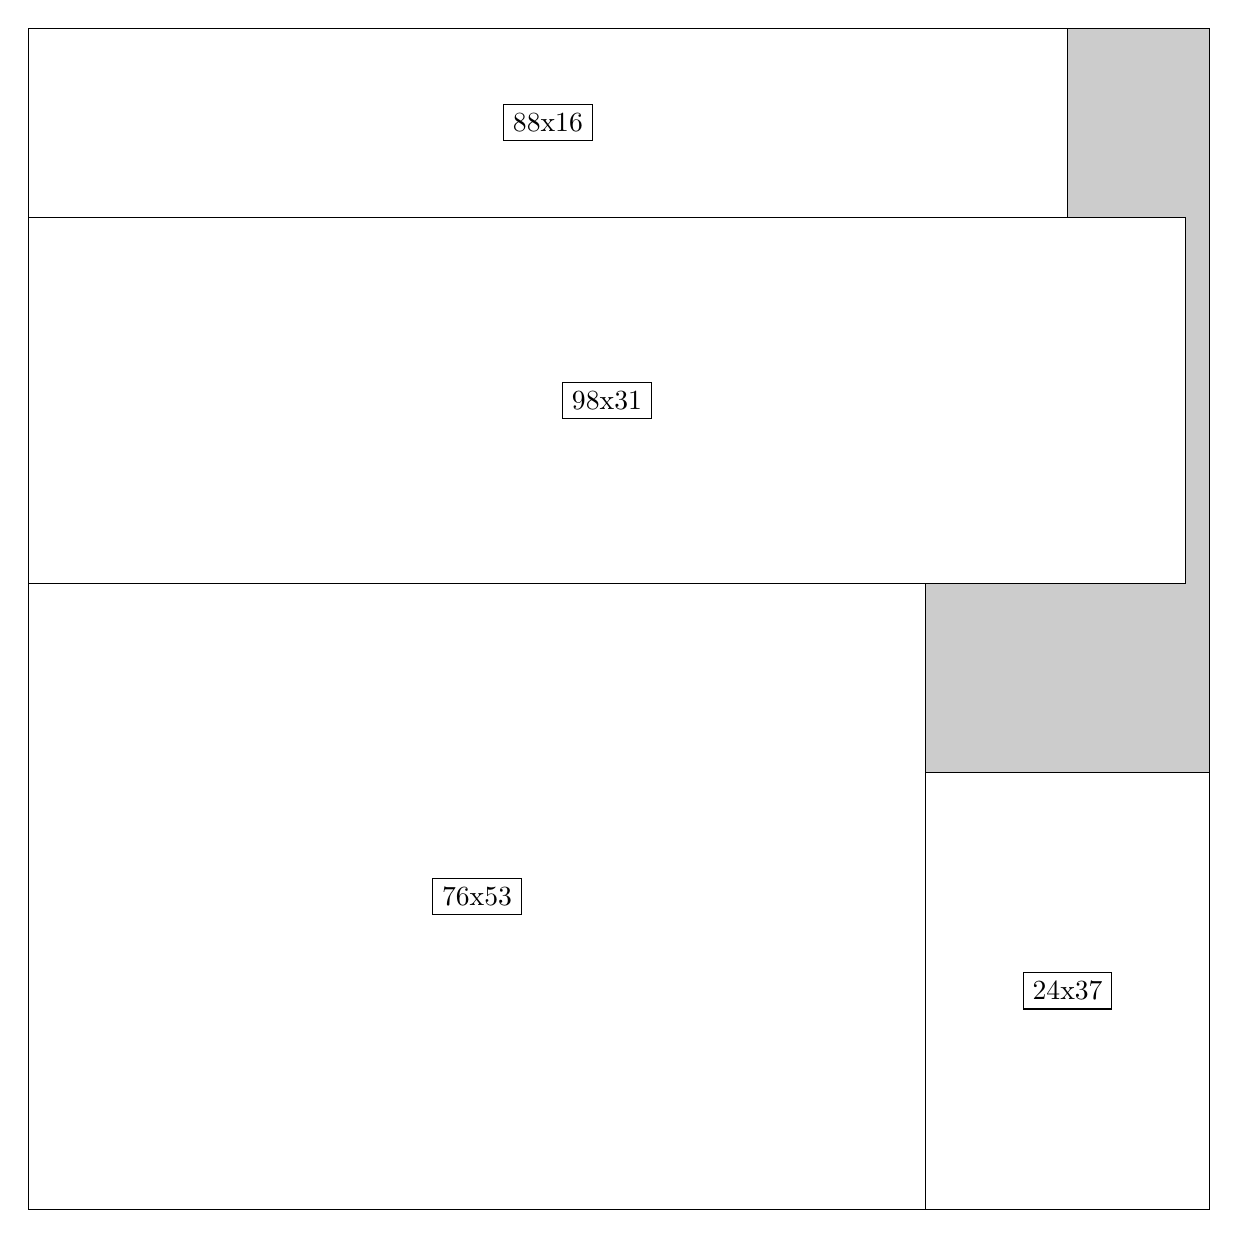
\begin{tikzpicture}[shorten >=1pt,scale=1.0,every node/.style={scale=1.0},->]
\tikzstyle{vertex}=[circle,fill=black!25,minimum size=14pt,inner sep=0pt]
\filldraw[fill=gray!40!white, draw=black] (0,0) rectangle (15.0,15.0);
\foreach \name/\x/\y/\w/\h in {76x53/0.0/0.0/11.4/7.949999999999999,98x31/0.0/7.949999999999999/14.7/4.6499999999999995,88x16/0.0/12.6/13.2/2.4,24x37/11.4/0.0/3.5999999999999996/5.55}
\filldraw[fill=white!40!white, draw=black] (\x,\y) rectangle node[draw] (\name) {\name} ++(\w,\h);
\end{tikzpicture}


w =76 , h =53 , x =0 , y =0 , v =4028
\par
w =98 , h =31 , x =0 , y =53 , v =3038
\par
w =88 , h =16 , x =0 , y =84 , v =1408
\par
w =24 , h =37 , x =76 , y =0 , v =888
\par
\newpage


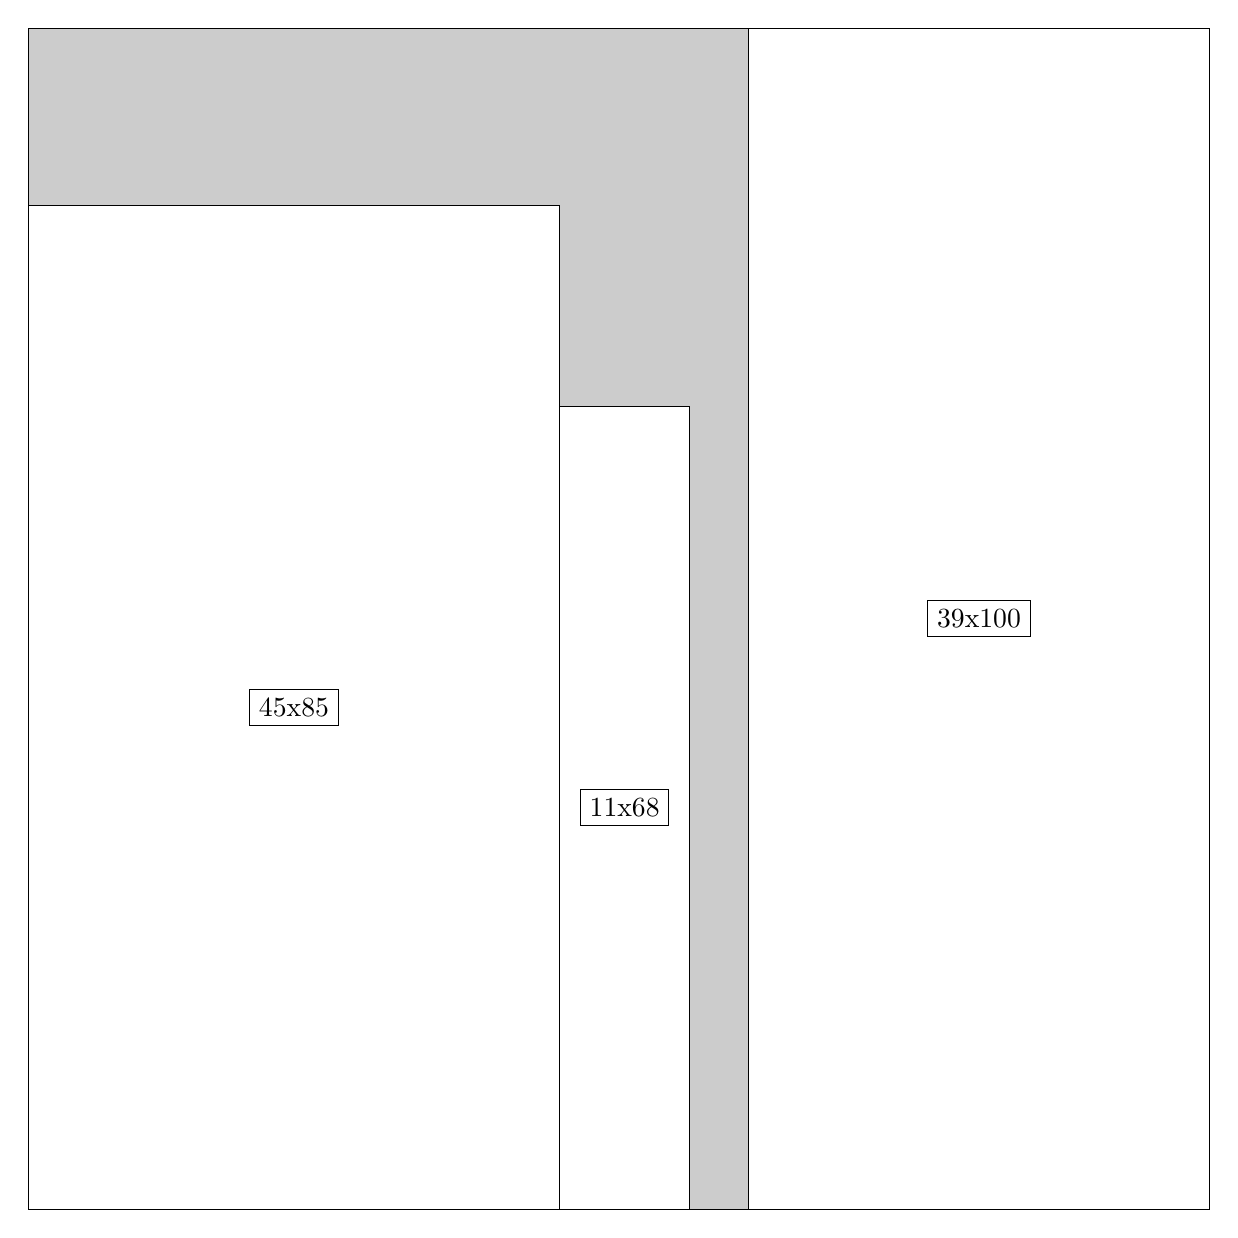
\begin{tikzpicture}[shorten >=1pt,scale=1.0,every node/.style={scale=1.0},->]
\tikzstyle{vertex}=[circle,fill=black!25,minimum size=14pt,inner sep=0pt]
\filldraw[fill=gray!40!white, draw=black] (0,0) rectangle (15.0,15.0);
\foreach \name/\x/\y/\w/\h in {39x100/9.15/0.0/5.85/15.0,45x85/0.0/0.0/6.75/12.75,11x68/6.75/0.0/1.65/10.2}
\filldraw[fill=white!40!white, draw=black] (\x,\y) rectangle node[draw] (\name) {\name} ++(\w,\h);
\end{tikzpicture}


w =39 , h =100 , x =61 , y =0 , v =3900
\par
w =45 , h =85 , x =0 , y =0 , v =3825
\par
w =11 , h =68 , x =45 , y =0 , v =748
\par
\newpage


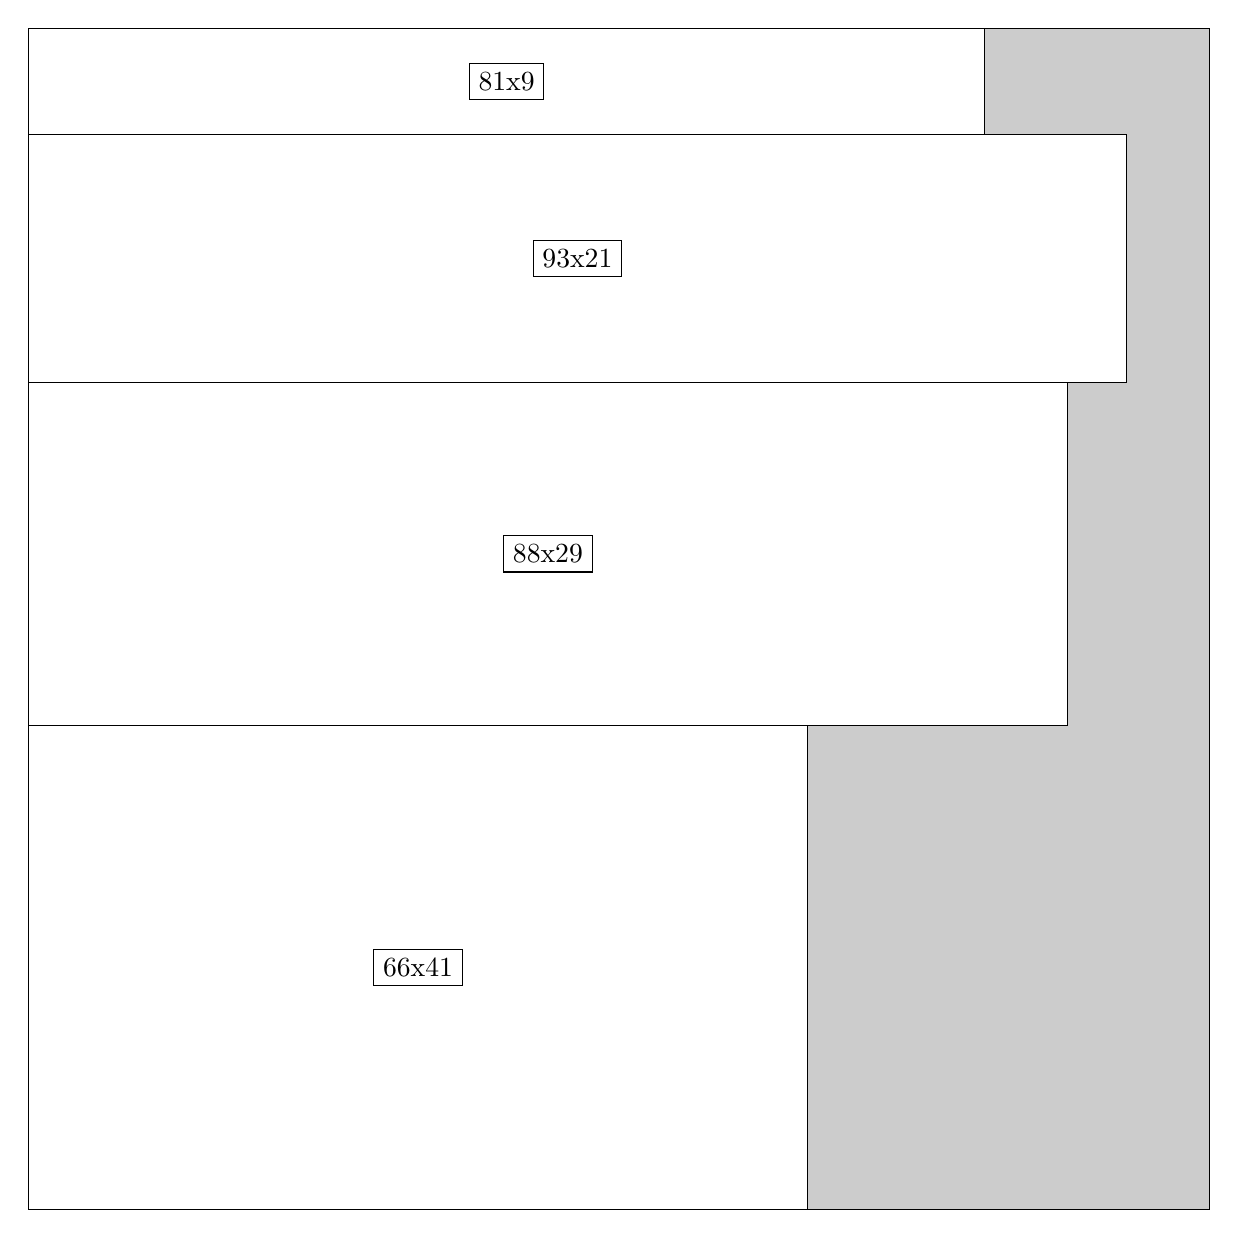
\begin{tikzpicture}[shorten >=1pt,scale=1.0,every node/.style={scale=1.0},->]
\tikzstyle{vertex}=[circle,fill=black!25,minimum size=14pt,inner sep=0pt]
\filldraw[fill=gray!40!white, draw=black] (0,0) rectangle (15.0,15.0);
\foreach \name/\x/\y/\w/\h in {66x41/0.0/0.0/9.9/6.1499999999999995,88x29/0.0/6.1499999999999995/13.2/4.35,93x21/0.0/10.5/13.95/3.15,81x9/0.0/13.65/12.15/1.3499999999999999}
\filldraw[fill=white!40!white, draw=black] (\x,\y) rectangle node[draw] (\name) {\name} ++(\w,\h);
\end{tikzpicture}


w =66 , h =41 , x =0 , y =0 , v =2706
\par
w =88 , h =29 , x =0 , y =41 , v =2552
\par
w =93 , h =21 , x =0 , y =70 , v =1953
\par
w =81 , h =9 , x =0 , y =91 , v =729
\par
\newpage


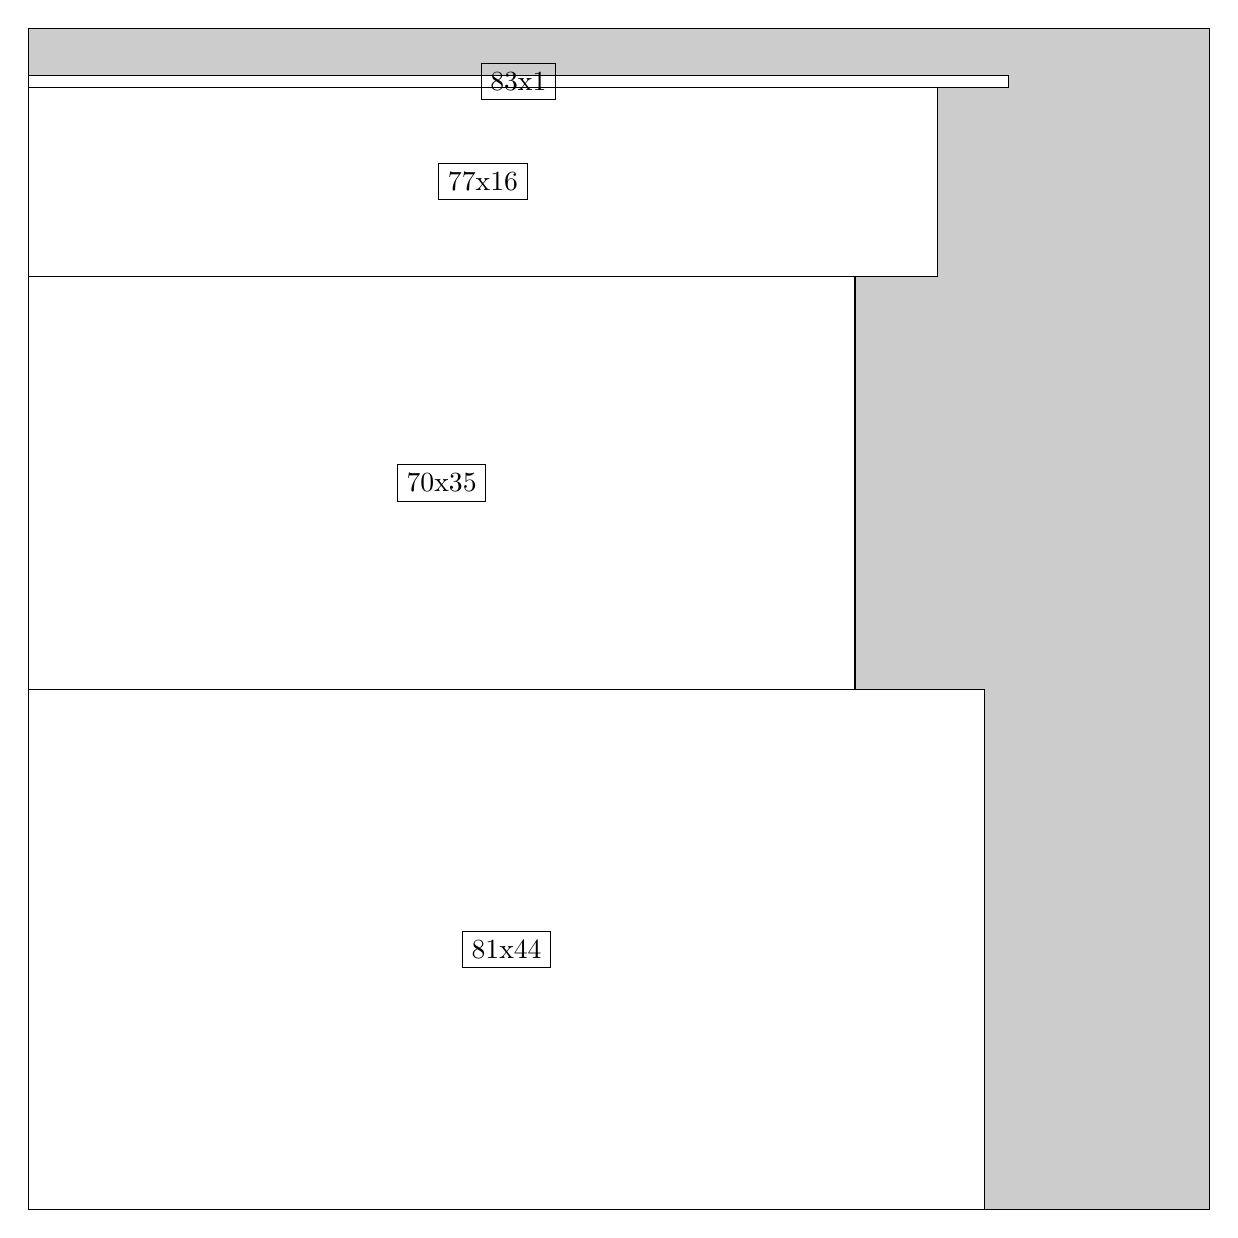
\begin{tikzpicture}[shorten >=1pt,scale=1.0,every node/.style={scale=1.0},->]
\tikzstyle{vertex}=[circle,fill=black!25,minimum size=14pt,inner sep=0pt]
\filldraw[fill=gray!40!white, draw=black] (0,0) rectangle (15.0,15.0);
\foreach \name/\x/\y/\w/\h in {81x44/0.0/0.0/12.15/6.6,70x35/0.0/6.6/10.5/5.25,77x16/0.0/11.85/11.549999999999999/2.4,83x1/0.0/14.25/12.45/0.15}
\filldraw[fill=white!40!white, draw=black] (\x,\y) rectangle node[draw] (\name) {\name} ++(\w,\h);
\end{tikzpicture}


w =81 , h =44 , x =0 , y =0 , v =3564
\par
w =70 , h =35 , x =0 , y =44 , v =2450
\par
w =77 , h =16 , x =0 , y =79 , v =1232
\par
w =83 , h =1 , x =0 , y =95 , v =83
\par
\newpage


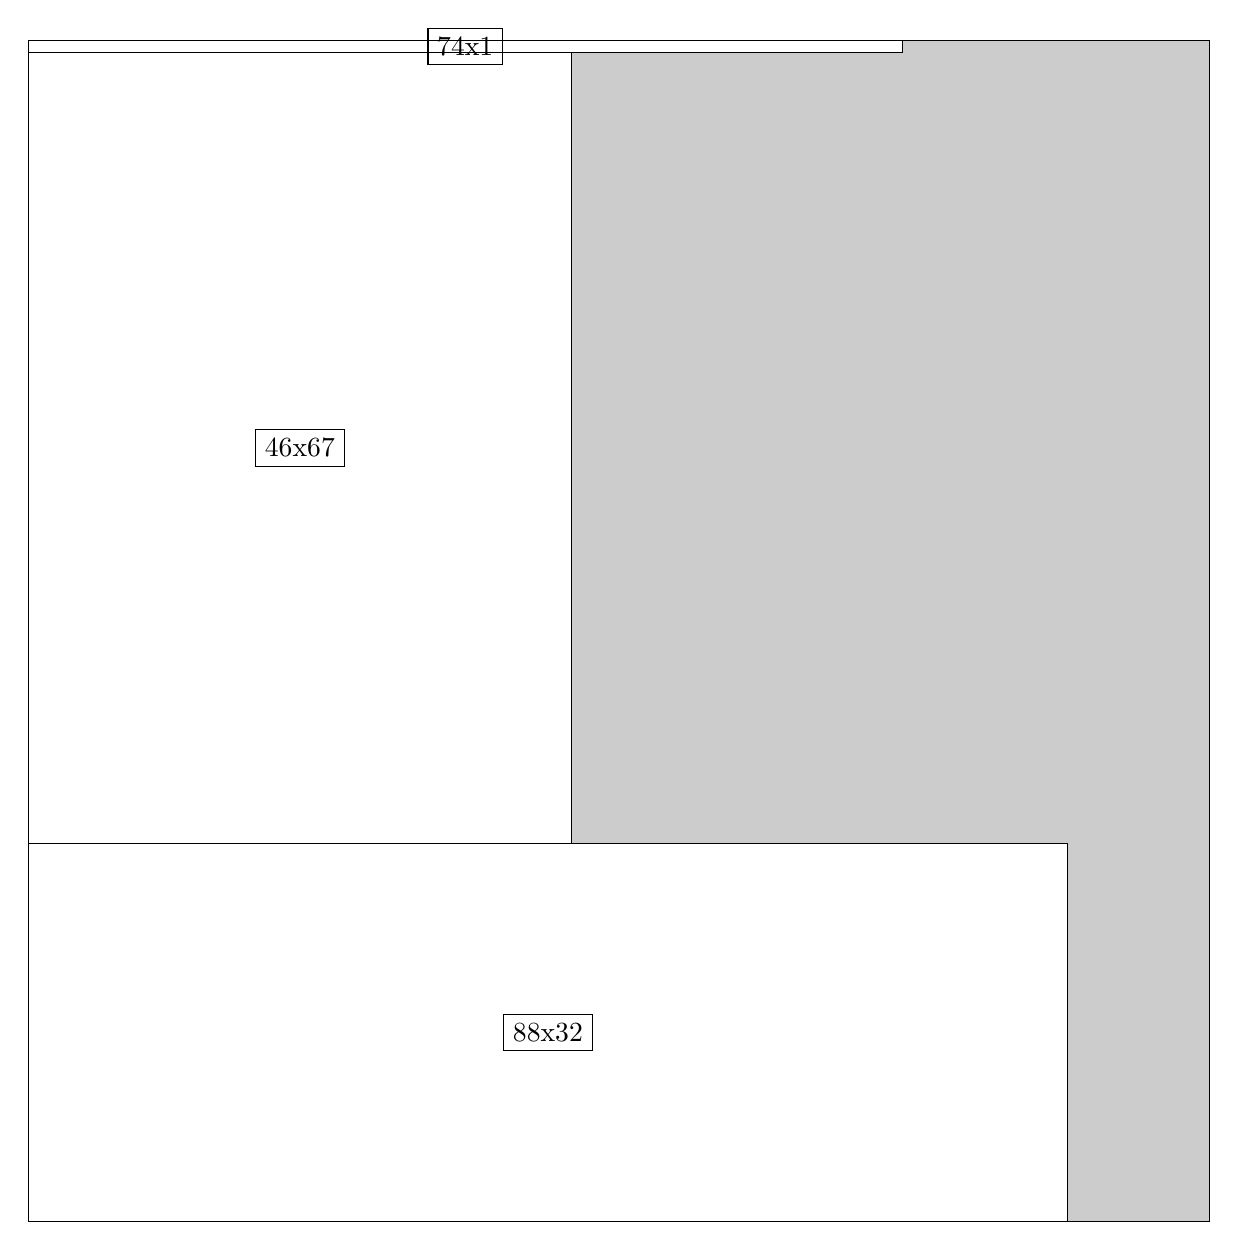
\begin{tikzpicture}[shorten >=1pt,scale=1.0,every node/.style={scale=1.0},->]
\tikzstyle{vertex}=[circle,fill=black!25,minimum size=14pt,inner sep=0pt]
\filldraw[fill=gray!40!white, draw=black] (0,0) rectangle (15.0,15.0);
\foreach \name/\x/\y/\w/\h in {88x32/0.0/0.0/13.2/4.8,46x67/0.0/4.8/6.8999999999999995/10.049999999999999,74x1/0.0/14.85/11.1/0.15}
\filldraw[fill=white!40!white, draw=black] (\x,\y) rectangle node[draw] (\name) {\name} ++(\w,\h);
\end{tikzpicture}


w =88 , h =32 , x =0 , y =0 , v =2816
\par
w =46 , h =67 , x =0 , y =32 , v =3082
\par
w =74 , h =1 , x =0 , y =99 , v =74
\par
\newpage


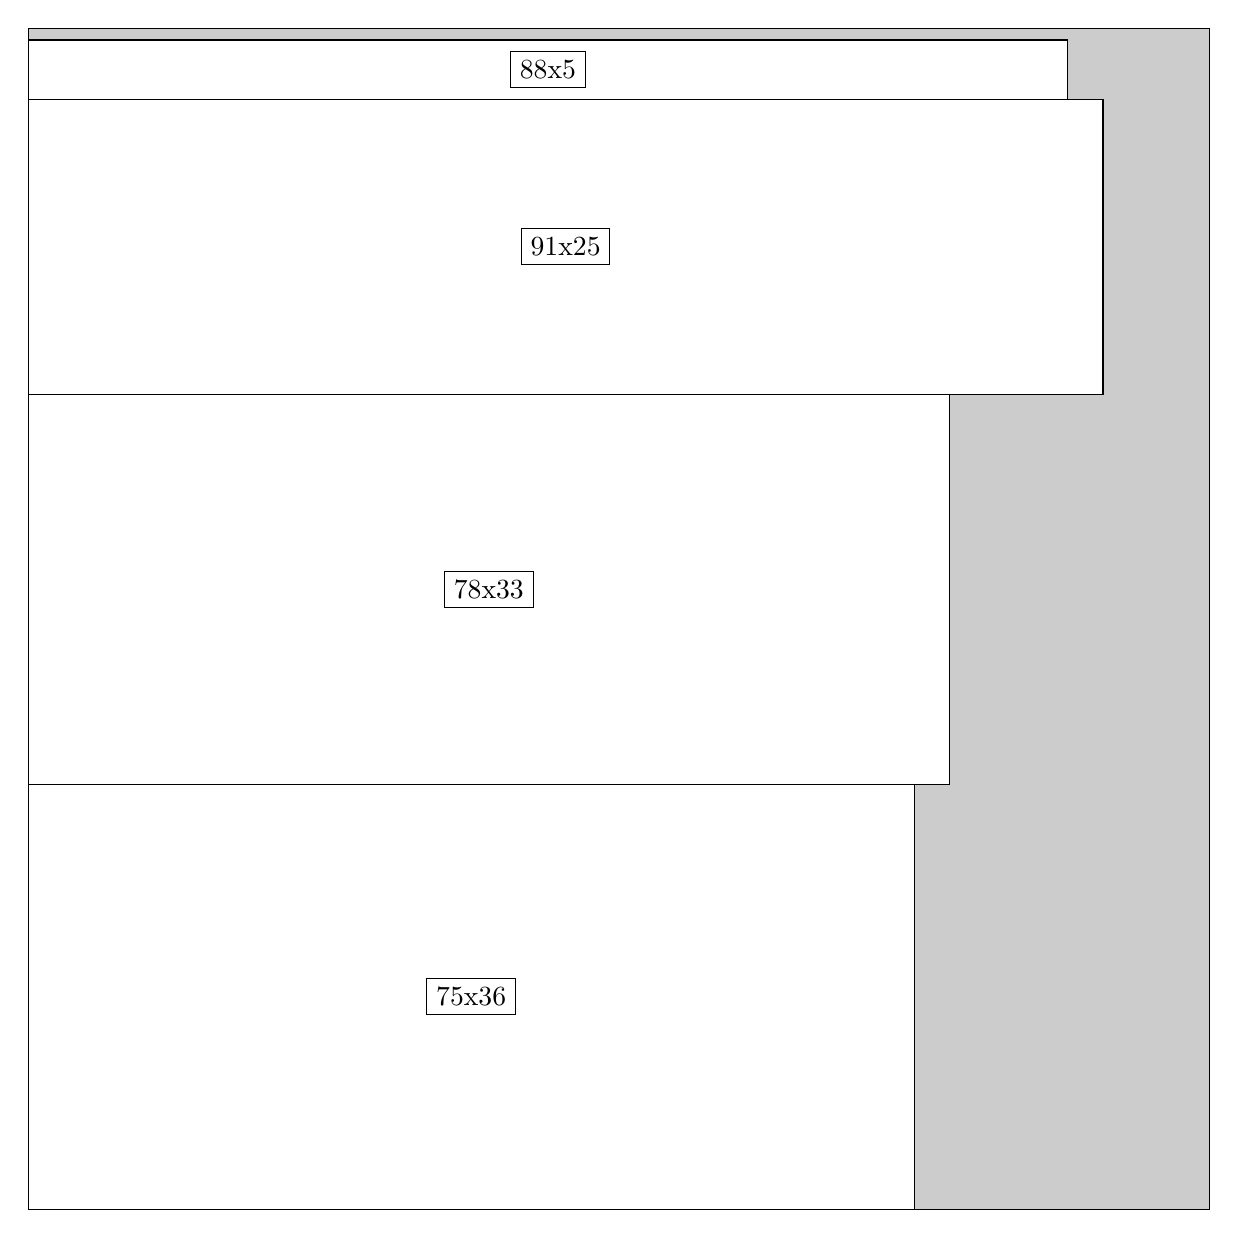
\begin{tikzpicture}[shorten >=1pt,scale=1.0,every node/.style={scale=1.0},->]
\tikzstyle{vertex}=[circle,fill=black!25,minimum size=14pt,inner sep=0pt]
\filldraw[fill=gray!40!white, draw=black] (0,0) rectangle (15.0,15.0);
\foreach \name/\x/\y/\w/\h in {75x36/0.0/0.0/11.25/5.3999999999999995,78x33/0.0/5.3999999999999995/11.7/4.95,91x25/0.0/10.35/13.65/3.75,88x5/0.0/14.1/13.2/0.75}
\filldraw[fill=white!40!white, draw=black] (\x,\y) rectangle node[draw] (\name) {\name} ++(\w,\h);
\end{tikzpicture}


w =75 , h =36 , x =0 , y =0 , v =2700
\par
w =78 , h =33 , x =0 , y =36 , v =2574
\par
w =91 , h =25 , x =0 , y =69 , v =2275
\par
w =88 , h =5 , x =0 , y =94 , v =440
\par
\newpage


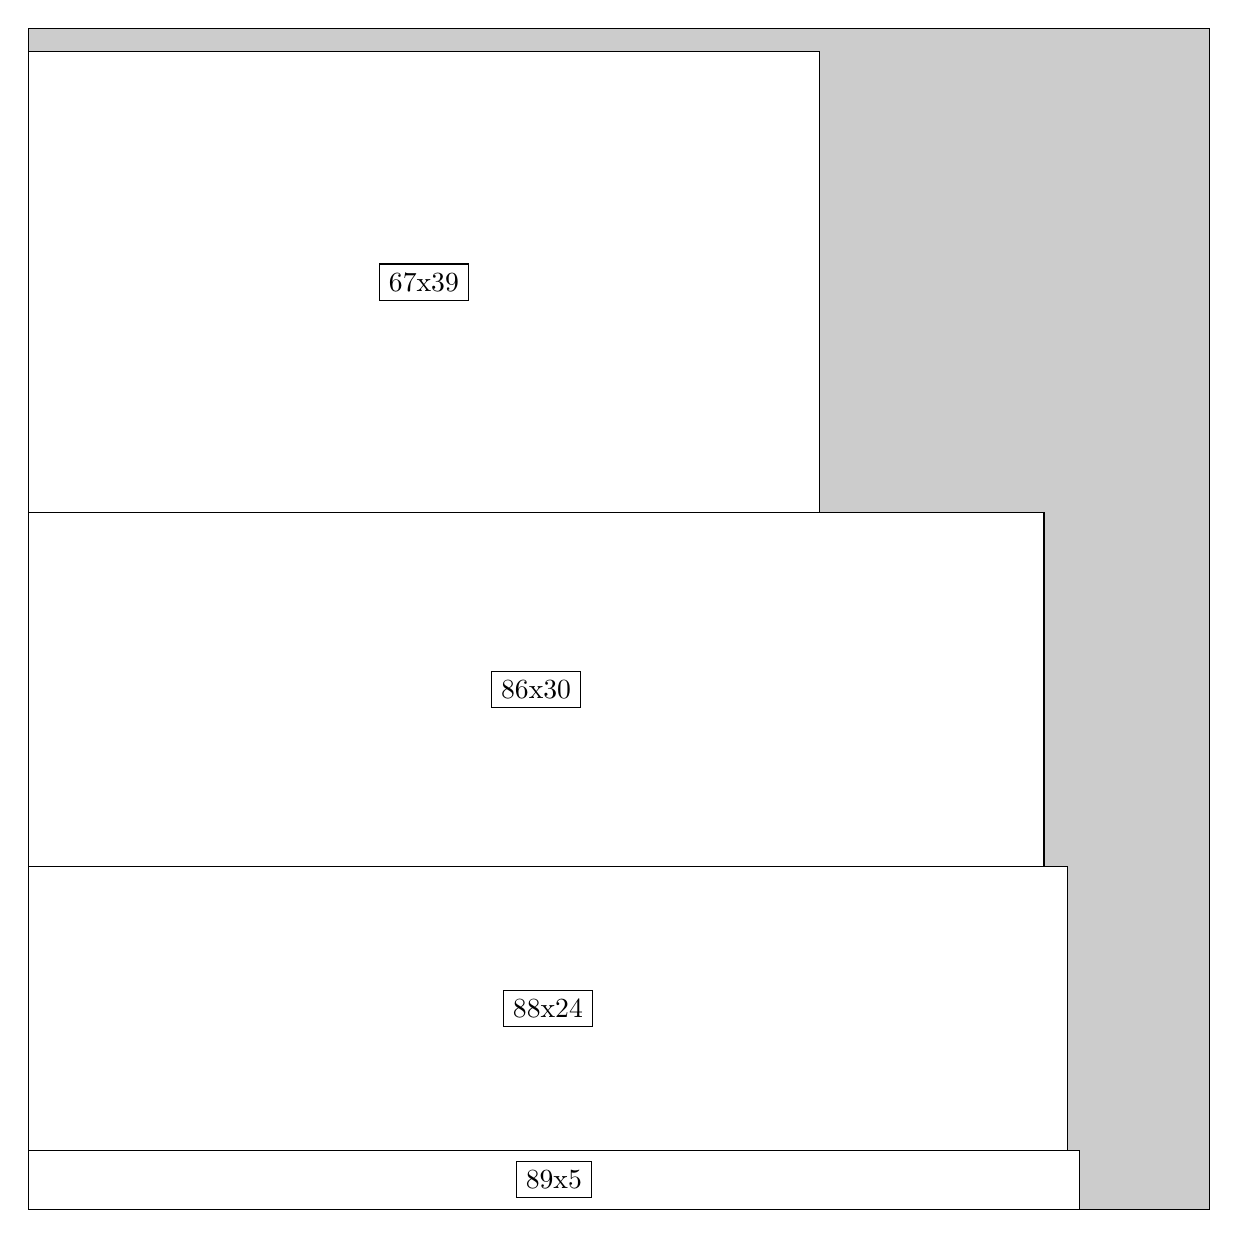
\begin{tikzpicture}[shorten >=1pt,scale=1.0,every node/.style={scale=1.0},->]
\tikzstyle{vertex}=[circle,fill=black!25,minimum size=14pt,inner sep=0pt]
\filldraw[fill=gray!40!white, draw=black] (0,0) rectangle (15.0,15.0);
\foreach \name/\x/\y/\w/\h in {67x39/0.0/8.85/10.049999999999999/5.85,86x30/0.0/4.35/12.9/4.5,88x24/0.0/0.75/13.2/3.5999999999999996,89x5/0.0/0.0/13.35/0.75}
\filldraw[fill=white!40!white, draw=black] (\x,\y) rectangle node[draw] (\name) {\name} ++(\w,\h);
\end{tikzpicture}


w =67 , h =39 , x =0 , y =59 , v =2613
\par
w =86 , h =30 , x =0 , y =29 , v =2580
\par
w =88 , h =24 , x =0 , y =5 , v =2112
\par
w =89 , h =5 , x =0 , y =0 , v =445
\par
\newpage


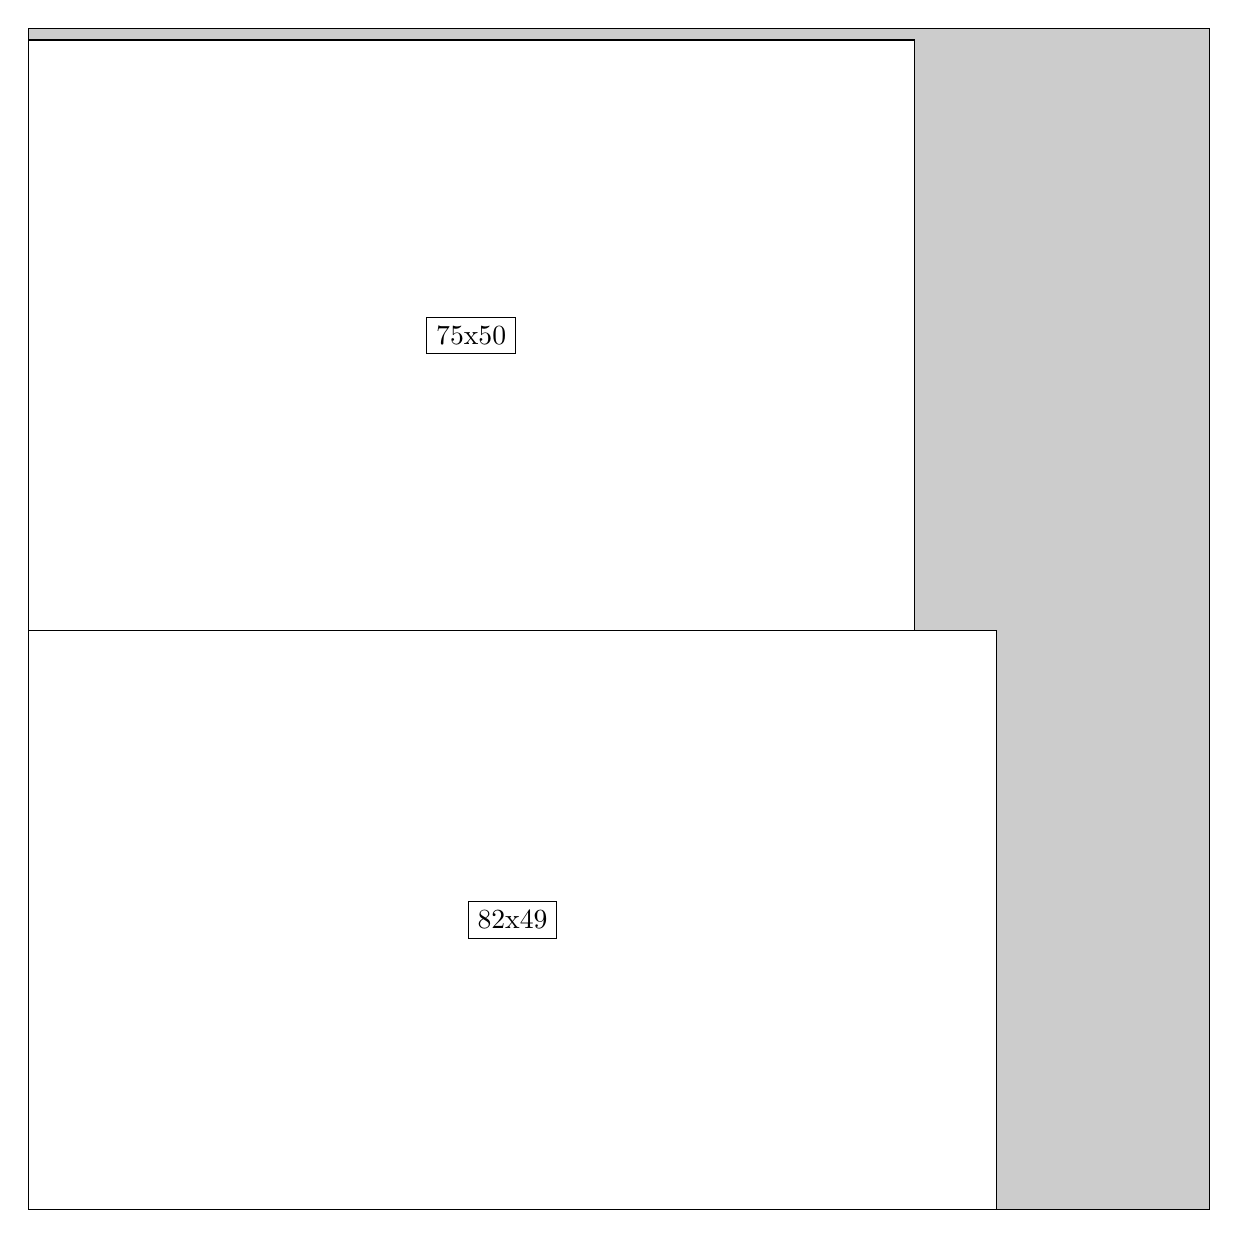
\begin{tikzpicture}[shorten >=1pt,scale=1.0,every node/.style={scale=1.0},->]
\tikzstyle{vertex}=[circle,fill=black!25,minimum size=14pt,inner sep=0pt]
\filldraw[fill=gray!40!white, draw=black] (0,0) rectangle (15.0,15.0);
\foreach \name/\x/\y/\w/\h in {82x49/0.0/0.0/12.299999999999999/7.35,75x50/0.0/7.35/11.25/7.5}
\filldraw[fill=white!40!white, draw=black] (\x,\y) rectangle node[draw] (\name) {\name} ++(\w,\h);
\end{tikzpicture}


w =82 , h =49 , x =0 , y =0 , v =4018
\par
w =75 , h =50 , x =0 , y =49 , v =3750
\par
\newpage


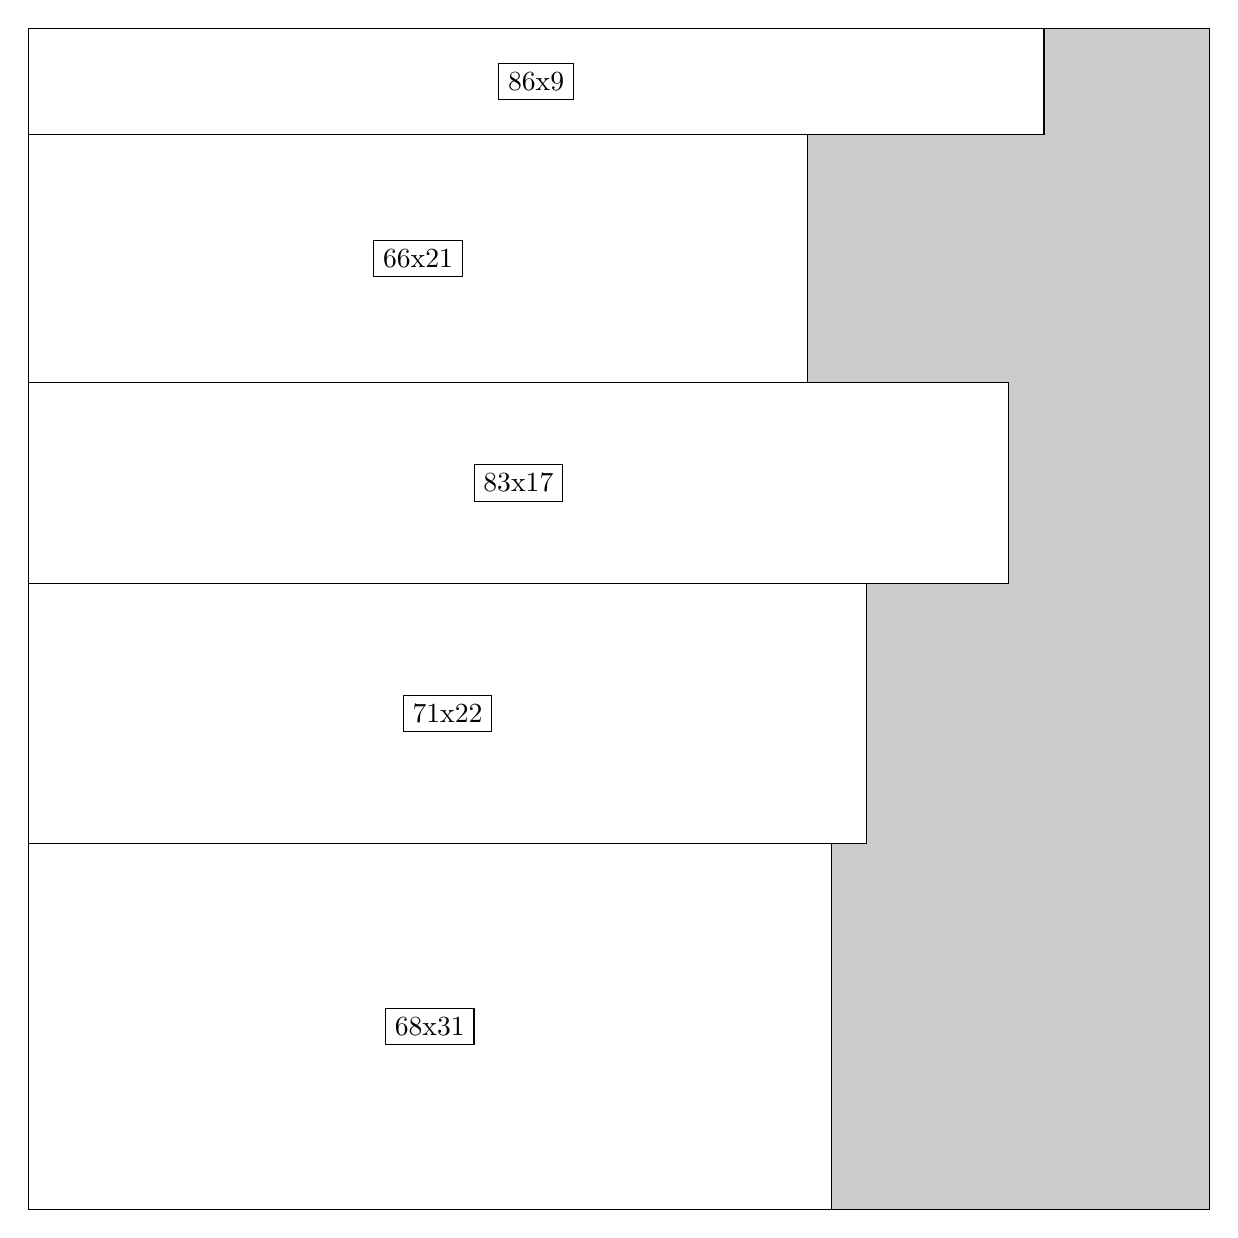
\begin{tikzpicture}[shorten >=1pt,scale=1.0,every node/.style={scale=1.0},->]
\tikzstyle{vertex}=[circle,fill=black!25,minimum size=14pt,inner sep=0pt]
\filldraw[fill=gray!40!white, draw=black] (0,0) rectangle (15.0,15.0);
\foreach \name/\x/\y/\w/\h in {68x31/0.0/0.0/10.2/4.6499999999999995,71x22/0.0/4.6499999999999995/10.65/3.3,83x17/0.0/7.949999999999999/12.45/2.55,66x21/0.0/10.5/9.9/3.15,86x9/0.0/13.65/12.9/1.3499999999999999}
\filldraw[fill=white!40!white, draw=black] (\x,\y) rectangle node[draw] (\name) {\name} ++(\w,\h);
\end{tikzpicture}


w =68 , h =31 , x =0 , y =0 , v =2108
\par
w =71 , h =22 , x =0 , y =31 , v =1562
\par
w =83 , h =17 , x =0 , y =53 , v =1411
\par
w =66 , h =21 , x =0 , y =70 , v =1386
\par
w =86 , h =9 , x =0 , y =91 , v =774
\par
\newpage


\end{document}